%%
%% Beginning of file 'sample62.tex'
%%
%% Modified 2018 January
%%
%% This is a sample manuscript marked up using the
%% AASTeX v6.2 LaTeX 2e macros.
%%
%% AASTeX is now based on Alexey Vikhlinin's emulateapj.cls 
%% (Copyright 2000-2015).  See the classfile for details.

%% AASTeX requires revtex4-1.cls (http://publish.aps.org/revtex4/) and
%% other external packages (latexsym, graphicx, amssymb, longtable, and epsf).
%% All of these external packages should already be present in the modern TeX 
%% distributions.  If not they can also be obtained at www.ctan.org.

%% The first piece of markup in an AASTeX v6.x document is the \documentclass
%% command. LaTeX will ignore any data that comes before this command. The 
%% documentclass can take an optional argument to modify the output style.
%% The command below calls the preprint style  which will produce a tightly 
%% typeset, one-column, single-spaced document.  It is the default and thus
%% does not need to be explicitly stated.
%%
%%
%% using aastex version 6.2
\documentclass{aastex62}

%% The default is a single spaced, 10 point font, single spaced article.
%% There are 5 other style options available via an optional argument. They
%% can be envoked like this:
%%
%% \documentclass[argument]{aastex62}
%% 
%% where the layout options are:
%%
%%  twocolumn   : two text columns, 10 point font, single spaced article.
%%                This is the most compact and represent the final published
%%                derived PDF copy of the accepted manuscript from the publisher
%%  manuscript  : one text column, 12 point font, double spaced article.
%%  preprint    : one text column, 12 point font, single spaced article.  
%%  preprint2   : two text columns, 12 point font, single spaced article.
%%  modern      : a stylish, single text column, 12 point font, article with
%% 		  wider left and right margins. This uses the Daniel
%% 		  Foreman-Mackey and David Hogg design.
%%  RNAAS       : Preferred style for Research Notes which are by design 
%%                lacking an abstract and brief. DO NOT use \begin{abstract}
%%                and \end{abstract} with this style.
%%
%% Note that you can submit to the AAS Journals in any of these 6 styles.
%%
%% There are other optional arguments one can envoke to allow other stylistic
%% actions. The available options are:
%%
%%  astrosymb    : Loads Astrosymb font and define \astrocommands. 
%%  tighten      : Makes baselineskip slightly smaller, only works with 
%%                 the twocolumn substyle.
%%  times        : uses times font instead of the default
%%  linenumbers  : turn on lineno package.
%%  trackchanges : required to see the revision mark up and print its output
%%  longauthor   : Do not use the more compressed footnote style (default) for 
%%                 the author/collaboration/affiliations. Instead print all
%%                 affiliation information after each name. Creates a much
%%                 long author list but may be desirable for short author papers
%%
%% these can be used in any combination, e.g.
%%
%% \documentclass[twocolumn,linenumbers,trackchanges]{aastex62}
%%
%% AASTeX v6.* now includes \hyperref support. While we have built in specific
%% defaults into the classfile you can manually override them with the
%% \hypersetup command. For example,
%%
%%\hypersetup{linkcolor=red,citecolor=green,filecolor=cyan,urlcolor=magenta}
%%
%% will change the color of the internal links to red, the links to the
%% bibliography to green, the file links to cyan, and the external links to
%% magenta. Additional information on \hyperref options can be found here:
%% https://www.tug.org/applications/hyperref/manual.html#x1-40003
%%
%% If you want to create your own macros, you can do so
%% using \newcommand. Your macros should appear before
%% the \begin{document} command.
%%

\usepackage{graphicx}
\usepackage{float}
\usepackage[caption=false]{subfig}
\usepackage{enumitem}

%\usepackage{natbib}
%\usepackage{pdflscape}

%% AASTeX v6.* now includes \hyperref support. While we have built in specific
%% defaults into the classfile you can manually override them with the
%% \hypersetup command. For example,
%%
%%\hypersetup{linkcolor=red,citecolor=green,filecolor=cyan,urlcolor=magenta}
%%
%% will change the color of the internal links to red, the links to the
%% bibliography to green, the file links to cyan, and the external links to
%% magenta. Additional information on \hyperref options can be found here:
%% https://www.tug.org/applications/hyperref/manual.html#x1-40003

%% If you want to create your own macros, you can do so
%% using \newcommand. Your macros should appear before
%% the \begin{document} command.
%%
\newcommand{\vdag}{(v)^\dagger}
\newcommand\aastex{AAS\TeX}
\newcommand\latex{La\TeX}
\newcommand{\exampleConstant}{0.04}
\newcommand{\degree}{^\circ}
\newcommand{\spitzer}{{\it Spitzer}}
\newcommand{\kepler}{{\it Kepler}}

%% Reintroduced the \received and \accepted commands from AASTeX v5.2
%\received{July 1, 2016}
%\revised{September 27, 2016}
%\accepted{\today}
%% Command to document which AAS Journal the manuscript was submitted to.
%% Adds "Submitted to " the arguement.
%\submitjournal{ApJ}

%% Mark up commands to limit the number of authors on the front page.
%% Note that in AASTeX v6.1 a \collaboration call (see below) counts as
%% an author in this case.
%
%\AuthorCollaborationLimit=3
%
%% Will only show Schwarz, Muench and "the AAS Journals Data Scientist 
%% collaboration" on the front page of this example manuscript.
%%
%% Note that all of the author will be shown in the published article.
%% This feature is meant to be used prior to acceptance to make the
%% front end of a long author article more manageable. Please do not use
%% this functionality for manuscripts with less than 20 authors. Conversely,
%% please do use this when the number of authors exceeds 40.
%%
%% Use \allauthors at the manuscript end to show the full author list.
%% This command should only be used with \AuthorCollaborationLimit is used.

%% The following command can be used to set the latex table counters.  It
%% is needed in this document because it uses a mix of latex tabular and
%% AASTeX deluxetables.  In general it should not be needed.
%\setcounter{table}{1}

%%%%%%%%%%%%%%%%%%%%%%%%%%%%%%%%%%%%%%%%%%%%%%%%%%%%%%%%%%%%%%%%%%%%%%%%%%%%%%%%
%%
%% The following section outlines numerous optional output that
%% can be displayed in the front matter or as running meta-data.
%%
%% If you wish, you may supply running head information, although
%% this information may be modified by the editorial offices.
\shorttitle{NIRCam Lab Studies}
\shortauthors{Schlawin et al.}
%%
%% You can add a light gray and diagonal water-mark to the first page 
%% with this command:
% \watermark{text}
%% where "text", e.g. DRAFT, is the text to appear.  If the text is 
%% long you can control the water-mark size with:
%  \setwatermarkfontsize{dimension}
%% where dimension is any recognized LaTeX dimension, e.g. pt, in, etc.
%%
%%%%%%%%%%%%%%%%%%%%%%%%%%%%%%%%%%%%%%%%%%%%%%%%%%%%%%%%%%%%%%%%%%%%%%%%%%%%%%%%

%% This is the end of the preamble.  Indicate the beginning of the
%% manuscript itself with \begin{document}.

\begin{document}

\title{Lessons Learned for JWST Transiting Planet Time Series from Ground-based Studies of NIRCam Detectors}

%% LaTeX will automatically break titles if they run longer than
%% one line. However, you may use \\ to force a line break if
%% you desire. In v6.1 you can include a footnote in the title.

%% A significant change from earlier AASTEX versions is in the structure for 
%% calling author and affilations. The change was necessary to implement 
%% autoindexing of affilations which prior was a manual process that could 
%% easily be tedious in large author manuscripts.
%%
%% The \author command is the same as before except it now takes an optional
%% arguement which is the 16 digit ORCID. The syntax is:
%% \author[xxxx-xxxx-xxxx-xxxx]{Author Name}
%%
%% This will hyperlink the author name to the author's ORCID page. Note that
%% during compilation, LaTeX will do some limited checking of the format of
%% the ID to make sure it is valid.
%%
%% Use \affiliation for affiliation information. The old \affil is now aliased
%% to \affiliation. AASTeX v6.1 will automatically index these in the header.
%% When a duplicate is found its index will be the same as its previous entry.
%%
%% Note that \altaffilmark and \altaffiltext have been removed and thus 
%% can not be used to document secondary affiliations. If they are used latex
%% will issue a specific error message and quit. Please use multiple 
%% \affiliation calls for to document more than one affiliation.
%%
%% The new \altaffiliation can be used to indicate some secondary information
%% such as fellowships. This command produces a non-numeric footnote that is
%% set away from the numeric \affiliation footnotes.  NOTE that if an
%% \altaffiliation command is used it must come BEFORE the \affiliation call,
%% right after the \author command, in order to place the footnotes in
%% the proper location.
%%
%% Use \email to set provide email addresses. Each \email will appear on its
%% own line so you can put multiple email address in one \email call. A new
%% \correspondingauthor command is available in V6.1 to identify the
%% corresponding author of the manuscript. It is the author's responsibility
%% to make sure this name is also in the author list.
%%
%% While authors can be grouped inside the same \author and \affiliation
%% commands it is better to have a single author for each. This allows for
%% one to exploit all the new benefits and should make book-keeping easier.
%%
%% If done correctly the peer review system will be able to
%% automatically put the author and affiliation information from the manuscript
%% and save the corresponding author the trouble of entering it by hand.

\correspondingauthor{Everett Schlawin}
\email{eas342 AT EMAIL Dot Arizona .edu}

\author[0000-0001-8291-6490]{Everett Schlawin}
\affiliation{Steward Observatory \\
933 North Cherry Avenue \\
Tucson, AZ 85721, USA}

\author{Jarron Leisenring}
\affiliation{Steward Observatory \\
933 North Cherry Avenue \\
Tucson, AZ 85721, USA}

\author{Karl Misselt}
\affiliation{Steward Observatory \\
933 North Cherry Avenue \\
Tucson, AZ 85721, USA}

\author{Rafia Bushra}
\affiliation{Steward Observatory \\
933 North Cherry Avenue \\
Tucson, AZ 85721, USA}

\author{Douglas Kelly}
\affiliation{Steward Observatory \\
933 North Cherry Avenue \\
Tucson, AZ 85721, USA} q

\author{Thomas Beatty}
\affiliation{Steward Observatory \\
933 North Cherry Avenue \\
Tucson, AZ 85721, USA}

\author{Stephanie Striegel}
\affiliation{Department of Physics \& Astronomy \\
San Jose State University \\
One Washington Square \\
San Jose, CA 95192, USA}
\affiliation{NASA Ames Research Center \\
Space Science and Astrobiology Division \\
Moffett Field, CA 94035, USA}

\author{Xander Levinson}
\affiliation{Department of Astronomy \& Astrophysics \\
University of California, Santa Cruz \\
1156 Highland Street \\
Santa Cruz, CA 95062, USA}
\affiliation{NASA Ames Research Center \\
Space Science and Astrobiology Division \\
Moffett Field, CA 94035, USA}

\author{Thomas P Greene}
\affiliation{NASA Ames Research Center \\
Space Science and Astrobiology Division \\
Moffett Field, CA 94035, USA}

\author{Marcia Rieke}
\affiliation{Steward Observatory \\
933 North Cherry Avenue \\
Tucson, AZ 85721, USA}


%% Note that the \and command from previous versions of AASTeX is now
%% depreciated in this version as it is no longer necessary. AASTeX 
%% automatically takes care of all commas and "and"s between authors names.

%% AASTeX 6.1 has the new \collaboration and \nocollaboration commands to
%% provide the collaboration status of a group of authors. These commands 
%% can be used either before or after the list of corresponding authors. The
%% argument for \collaboration is the collaboration identifier. Authors are
%% encouraged to surround collaboration identifiers with ()s. The 
%% \nocollaboration command takes no argument and exists to indicate that
%% the nearby authors are not part of surrounding collaborations.

%% Mark off the abstract in the ``abstract'' environment. 
\begin{abstract}

JWST transmission and emission spectra of transiting exoplanets will provide invaluable glimpses at exoplanet atmospheres that reveal the composition and temperature structure at a level never achieved before.
This promising science from JWST, however, will require exquisite precision and understanding of systematic errors that can impact the time series of planets crossing in front of and behind their host stars.
This is especially true if JWST is used to search for biosignatures in temperature atmospheres on Earth-sized planets that may contain liquid water.
Here, we provide the lessons learned from ground-based characterization of the NIRCam H2RG detectors, which will be used for exoplanet spectra and are the same type of detectors used in JWST's NIRISS and NIRSpec instruments.
We summarize the lessons learned from cryogenic vacuum campaigns 2 and 3 at NASA Goddard and the full telescope element at NASA Johnson with the flight hardware, as well as laboratory tests of the same detectors at the University of Arizona's Steward Observatory.

\end{abstract}

%% Keywords should appear after the \end{abstract} command. 
%% See the online documentation for the full list of available subject
%% keywords and the rules for their use.
\keywords{stars: atmospheres --- stars: individual (\objectname{KIC 12557548}) ---
stars: variables: general}

%% From the front matter, we move on to the body of the paper.
%% Sections are demarcated by \section and \subsection, respectively.
%% Observe the use of the LaTeX \label
%% command after the \subsection to give a symbolic KEY to the
%% subsection for cross-referencing in a \ref command.
%% You can use LaTeX's \ref and \label commands to keep track of
%% cross-references to sections, equations, tables, and figures.
%% That way, if you change the order of any elements, LaTeX will
%% automatically renumber them.

%% We recommend that authors also use the natbib \citep
%% and \citet commands to identify citations.  The citations are
%% tied to the reference list via symbolic KEYs. The KEY corresponds
%% to the KEY in the \bibitem in the reference list below. 

\section{Introduction} \label{sec:intro}

JWST will provide powerful new measurements of exoplanet atmospheres with spectroscopy from 0.6 to 12 $\mu$m
\citep{beichman2014pasp,greene2016jwst_trans,howe2017informationJWST,barstow2015jwstSystematics,schlawin2018JWSTforecasts}.
The sensitivity of JWST combined with its unprecedented wavelength coverage on exoplanets will enable it to measure the abundance of carbon-bearing molecules (CO, CO$2$ and CH$_4$) as well as study cooler, smaller planets than previously characterized.

JWST has also been considered for observations of temperate Earth-like planets that orbit their stars at a distance where where water could be in liquid form on their surface.
The TRAPPIST-1 system \citep{gillon2016trappist1Discovery,gillon2017trappist-1sevenp} presents an exciting opportunity to study Earth-sized stars orbiting a 0.1~R$_\odot$ M-type star.
By putting together 10-30 transits, it will be possible to collect enough photons to detect CO$_2$ \citep{barstow2016trappist1habitable,krissansen-totton2018trappist1eJWST} and, optimistically, O$_3$ in the atmosphere of TRAPPIST-1 d with JWST if clouds have a minimal impact to its atmosphere \citep{barstow2016trappist1habitable}.
A critical question in studying a planet like TRAPPIST-1 d, however, is whether photon-limited performance is possible with JWST observations.

Experience with the Hubble Space Telescope (HST), \spitzer, and \kepler\ shows that many systematics can affect high precision time series and prevent photon-limited performance unless corrected for \citep[e.g.][]{beichman2014pasp}.
Many of these effects are detector-related including charge trapping on HST's detector \citep{berta2012flat_gj1214,zhou2017chargeTrap}, intra-pixel sensitivity on the short wavelength bands of \spitzer\ IRAC \citep{moralesCalderon2006LdwarfsWeatherIPC} and sensitivity to pointing jitter with \kepler\footnote{https://keplerscience.arc.nasa.gov/K2/Performance.shtml} \citep{beichman2014pasp}.

The NIRCam instrument \citep{rieke2005nircamSPIE} contains a slitless grism mode \citep{greene2017jatisNIRCam} that is analogous to the WFC3 grism mode on HST that has been successfully employed on many transiting planets \citep[e.g.]{deming13,kreidberg2014wasp43,sing2016continuum,wakeford2017hatp26}.
The grism mode will collect moderate resolution R$\sim$1100-1700 spectra and employ the long wavelength channel to cover the wavelength range 2.4 to 5.0~$\mu$m.
This grism mode can be used simultaneously with short wavelength weak lens imaging or the Dispersed Hartmann Sensor mode \citep{schlawin2017dhs}. If it becomes an approved and implemented mode, the DHS will permit spectroscopy from 1.0 to 2.0~$\mu$m and will work for very bright targets inaccessible by other modes.

Section \ref{sec:experiments} describes the experiments on the ground that are used to prepare for JWST observations in flight.

\section{Known Detector Effects}
Known detector effects that could affect stability include:
\begin{itemize}[noitemsep]
	\item Intrapixel sensitivity - including sub-pixel flat fielding issues and sub-pixel crosshatching on the detectors \citep{shapiro2018crosshatch}
	\item Pre-amp reset offsets (an Asic-related effect) The NIRCam detectors' pre-amps are reset once per frame (as opposed to once per integration) to prevent large amplifier drifts over an integration \citep{robberto2014refPixPreAmp}.
The resets cause discontinuities in the (bias?) level that can be seen on reference pixels.
The NIRCam grism subarrays include reference pixels to mitigate these pre-amp offsets.
	\item 1/f noise - this is a noise source where most of the noise power is concentrated as low frequencies. 1/f noise causes spatial correlations in the fast-read direction (along detector rows). It is highly correlated between amplifiers, suggesting that it is caused by a common reference voltage. 1/f noise is efficiently removed by reference pixels
	\item Even/odd offsets - alternating columns have different bias levels. Additionally, there are offsets between columns that can change from frame to frame, especially on NIRCam's LW detector
	\item kTC noise - a random process due to the unknown amount of charge stored at the reset voltage level
\end{itemize}

\begin{figure}[!hbtp]
\centering
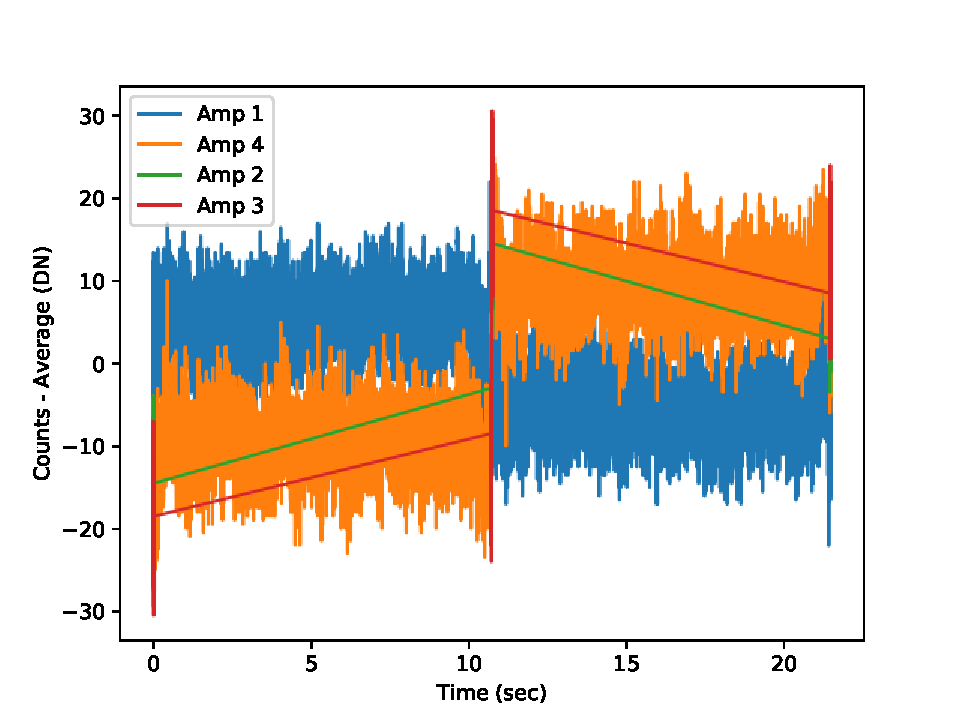
\includegraphics[width=.4\columnwidth]{allamps.pdf}
\caption{Reference pixel time series for a two ramp integration showing pre-amplifier resets.}\label{fig:sampFig}
\end{figure}

allamps.pdf

\section{Ground-based Experiments}\label{sec:experiments}

Table \ref{tab:testSummary} shows a summary of the ground-based tests that were performed on NIRCam detectors.
The flight NIRCam detectors, controllers, electronics, optics and instrument hardware were used in the Cryogenic Vacuum Test 3 (CV3) as well as OTIS (Optical Telescope Element and Integrated Science).
The GL dewar experiments used flight detectors, but a different controller (Leach).
The Asic dewar located at Steward Observatory in Tucson, Arizona used a spare NIRCam detector, a spare asic controller and the flight software, but no flight optics.

The instrument modes tested included mostly imaging with narrowband LEDs, but there was also a test with spectroscopy on a broadband source.
The WLP8 imaging tests are where a point source is de-focused by 8 waves with a weak lens (WLP8).
This mode was designed for wavefront sensing, but is also useful for high-precision time series because it spreads the light over many pixels.
The weak lens produces a point spread function (PSF) that is hexagonal like JWST's mirrors and has a flat-to-flat width of $\sim$108 pixels and a vertex-to-vertex width of $\sim$136 pixels.
The hexagonal PSF also has a central vertical peak which can be used for aperture centering.
The tests with dewars did not have NIRCam optics and instead were flood illuminated with a light source that had large spatial variations due to a non-uniform source.
One of the stability tests during the OTIS test at NASA Johnson was a grism spectroscopy mode that used the F322W2 to illuminate the detector with a slitless spectrum covering 2.4 to 4.0~$\mu$m.
 
\begin{deluxetable*}{ccCrlc}[b!]
\tablecaption{Summary of Ground-Based Tests}\label{tab:testSummary}
\tablecolumns{7}
%\tablenum{2}
\tablewidth{0pt}
\tablehead{
\colhead{Name} &
\colhead{Location} &
\colhead{UT dates} &
\colhead{Best Stability} & 
\colhead{Light Source} & 
\colhead{Instrument Mode} \\
\colhead{} &
\colhead{} &
\colhead{(YYYY-mm-dd)} &
\colhead{(ppm)} &
\colhead{}
}
\startdata
CV 3       & NASA Goddard  & 2016       & 500   	& LED           & WLP8 imaging \\
OTIS       & NASA Johnson  & 2017       &   2200    	& Continuum     & Grism spectroscopy \\
OTIS       & NASA Johnson  & 2017       &   21,000    	& Continuum     & WLP8 Imaging \\
GL dewar   & Steward Obs.  & 2015-2016  &       	& LED	        & flood-illuminated imaging \\
Asic dewar & Steward Obs.  & 2017-2019  &       	& LED           & pinhole flood-illuminated imaging \\
\enddata
\tablecomments{Cryogenic vacuum (CV).}
\end{deluxetable*}




\section{Figures\label{sec:figures}}

Figure \ref{fig:sampFig} shows a sample figure on its own.
Figure \ref{fig:gridFig} shows a grid figure.



\subsection{Grid Figures}\label{sec:gridFig}

%\begin{figure*}
%\gridline{\fig{sample_img.pdf}{0.3\textwidth}{Red Figure}
%          \fig{sample_red.png}{0.3\textwidth}{Green Figure}
%          }
%\caption{Two figures side by side.\label{fig:gridFig}}
%\end{figure*}


%% If you wish to include an acknowledgments section in your paper,
%% separate it off from the body of the text using the \acknowledgments
%% command.
\acknowledgments

\section*{acknowledgements}
MCMC fitting makes use of \texttt{emcee} \citep{foreman-mackey2013emcee} and the covariance plot was made with \texttt{corner.py} \citep{foremanCorner}.
Funding for the E Schlawin is provided by NASA Goddard Spaceflight Center.
This research has made
use of the Exoplanet Orbit Database and the Exoplanet Data Explorer at \url{http://exoplanets.org}; SIMBAD database, operated at CDS, Strasbourg,
France; NASA'��s Astrophysics Data System Bibliographic
Services; the M, L, T, and Y dwarf compendium
housed at \url{http://DwarfArchives.org}; the SpeX Prism
Libraries at \url{http://www.browndwarfs.org/spexprism}; and the \texttt{astropy} package \citep{astropy2013}. 
The authors wish to recognize and acknowledge the very significant cultural role and reverence that the summit of Mauna Kea has always had within the indigenous Hawaiian community. We are most fortunate to have the opportunity to conduct observations from this mountain.

%% To help institutions obtain information on the effectiveness of their 
%% telescopes the AAS Journals has created a group of keywords for telescope 
%% facilities.
%
%% Following the acknowledgments section, use the following syntax and the
%% \facility{} or \facilities{} macros to list the keywords of facilities used 
%% in the research for the paper.  Each keyword is check against the master 
%% list during copy editing.  Individual instruments can be provided in 
%% parentheses, after the keyword, but they are not verified.

\vspace{5mm}
\facilities{HST(WFC3), IRTF(SpeX)}

%% Similar to \facility{}, there is the optional \software command to allow 
%% authors a place to specify which programs were used during the creation of 
%% the manusscript. Authors should list each code and include either a
%% citation or url to the code inside ()s when available.

\software{astropy \citep{astropy2013}, 
          \texttt{emcee} \citep{foreman-mackey2013emcee}, 
          \texttt{batman} \citep{kreidberg2015batman},
          \texttt{spiderman} \citep{louden2017spiderman},
          \texttt{pynrc} \url{https://github.com/JarronL/pynrc},
          \texttt{emcee} \citep{foreman-mackey2013emcee}
           }

%% Appendix material should be preceded with a single \appendix command.
%% There should be a \section command for each appendix. Mark appendix
%% subsections with the same markup you use in the main body of the paper.

%% Each Appendix (indicated with \section) will be lettered A, B, C, etc.
%% The equation counter will reset when it encounters the \appendix
%% command and will number appendix equations (A1), (A2), etc. The
%% Figure and Table counter will not reset.

\appendix

%\section{Extra Info}

%% The reference list follows the main body and any appendices.
%% Use LaTeX's thebibliography environment to mark up your reference list.
%% Note \begin{thebibliography} is followed by an empty set of
%% curly braces.  If you forget this, LaTeX will generate the error
%% "Perhaps a missing \item?".
%%
%% thebibliography produces citations in the text using \bibitem-\cite
%% cross-referencing. Each reference is preceded by a
%% \bibitem command that defines in curly braces the KEY that corresponds
%% to the KEY in the \cite commands (see the first section above).
%% Make sure that you provide a unique KEY for every \bibitem or else the
%% paper will not LaTeX. The square brackets should contain
%% the citation text that LaTeX will insert in
%% place of the \cite commands.

%% We have used macros to produce journal name abbreviations.
%% \aastex provides a number of these for the more frequently-cited journals.
%% See the Author Guide for a list of them.

%% Note that the style of the \bibitem labels (in []) is slightly
%% different from previous examples.  The natbib system solves a host
%% of citation expression problems, but it is necessary to clearly
%% delimit the year from the author name used in the citation.
%% See the natbib documentation for more details and options.

\bibliographystyle{apj}
\bibliography{this_biblio}

%% This command is needed to show the entire author+affilation list when
%% the collaboration and author truncation commands are used.  It has to
%% go at the end of the manuscript.
%\allauthors

%% Include this line if you are using the \added, \replaced, \deleted
%% commands to see a summary list of all changes at the end of the article.
%\listofchanges

\end{document}

% End of file `sample61.tex'.
